\section{Guide utilisateur}
Dans cette section, nous allons vous guider sur la prise main de l'ensemble du projet.
Nous allons vous expliquer comment utiliser le modèle QDF dans les grandes lignes en une série d'étapes pour assurer la cohérence de la pipeline et prédire les propriétés des matériaux donneurs, en particulier le PCE. 
En ce qui concerne l'explication du code des notebooks au format \texttt{.ipynb} ainsi que les commentaires présents dans le code, ont été mis à disposition pour comprendre le fonctionnement de ce derniers.
Aussi,  nous nous accentuerons sur les traitements des deux datasets principaux que sont les PM (polymers molecules) et les SM (small molecules) et comment on parvient à les utiliser dans le modèle.\\
\textbf{NB } : On tient à rappeler que l'ensemble des commandes qui seront présentées par la suite ont été effectuées sur windows.

\subsection{Arbre du projet}

L'Arbre du projet est organisé de manière à faciliter la navigation et l'utilisation des différents composants du projet. Voici un aperçu de la structure de l'arborescence : 

\begin{figure}[H]
    \centering
    \begin{minipage}{0.2\linewidth}
        \begin{forest}
            pic dir tree,
            where level=0{}{% folder icons by default; override using file for file icons
                directory,
            },
            [ProjetDonor
              [data\_preprocess
                [coordinates.py, file]
                [coordinates.sh, file]
                [split\_data.py, file]
                [split\_data.sh, file]
              ]
              [datasets
                [output]
                [data\_test]
                [PM]
                [SM]
              ]
              [model
                [predict]
                [preprocess]
                [train\_model]
              ]
              [VAE]
              [requirements.txt, file]
              [courbe\_apprentissage.py, file]
              [output\_SM.txt ou output\_PM.txt, file]
            ]
          \end{forest}
\end{minipage}
\caption{Arborescence du projet}
\label{fig:arborescence}
\end{figure}

\paragraph{Data\_preprocess :} 
Le dossier \texttt{data\_preprocess} contient les scripts nécessaires pour prétraiter les données. 
En effet, la forme principale des molécules des datasets pour les PM (polymers molecules) et SM (small molecules) sont au format \textbf{SMILES} il va donc falloir les traiter pour les passer sous forme de coordonnées 3D en utilisant \textbf{RdKit}.

\paragraph{Datasets :}
Le dossier \texttt{datasets} contient les dossiers \texttt{PM} et \texttt{SM} eux même qui contiennent chacun les datasets (des PM et SM) encodés sous forme SMILES et les coordonnées 3D associées à ces datasets pour l'entrainement, la validation et le test.
Le dossier \texttt{output} contient les résultats de la prédiction du PCE pour les PM et SM ainsi que les modèles d'entrainement associés.

\paragraph{Model :}
Le dossier \texttt{model} contient les scripts nécessaires pour l'entrainement du modèle QDF, la prédiction du PCE et le preprocess des données réalisés sur les datasets PM.csv et SM.csv.

% \paragraph{VAE :}
% djeci

Avant de commencer à expliquer les principales étapes du projet, il est important de prendre en compte le fait qu'au départ seuls les dossiers \texttt{PM} et \texttt{SM} contenant les fichiers \texttt{PM.csv} et \texttt{SM.csv} sont contenus dans le dossiers datasets. 
Au fur et à mesure qu'on effectue les étapes la strucutre change en rajoutant des dossiers.

\subsection{Séparation du dataset}

La première étape du projet consiste à réaliser une séparation du dataset (PM.csv ou SM.csv) que l'on veut utiliser en trois parties : une partie pour l'entrainement, une partie pour la validation et une partie pour le test.
Pour cela on utilise le script \texttt{split\_data.sh} qui se trouve dans le dossier \texttt{data\_preprocess}.
\\
Le contenu du script \texttt{split\_data.sh} est le suivant :
\begin{figure}[htbp]
    \centering
    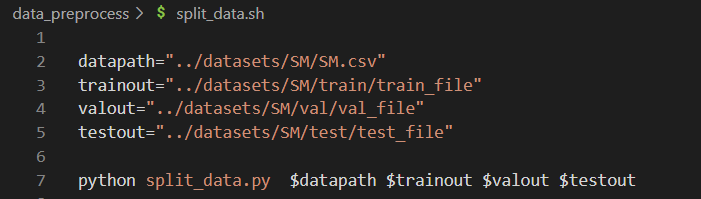
\includegraphics[width=0.6\textwidth]{GuideUtilisateur/split1.png}
    \caption{Contenu du script split\_data.sh}
\end{figure}

Dans cette image on peut voir que l'on utilise le script \texttt{split\_data.py} qui se trouve dans le même dossier. Le premier argument (datapath) est le nom du fichier CSV à traiter (PM.csv ou SM.csv) et les autres arguments sont les noms des des dossiers de sortie.

Pour exécuter le script, il faut ouvrir un terminal \textbf{bash} sur un éditeur comme VS code, accéder au dossier data\_preprocess avec la commande \texttt{cd data\_preprocess} et lancer le scritpt depuis ce terminal avec la commande : \texttt{bash split\_data.sh} sur windows. \\
\textbf{NB} : Si on veut fait un split des données sur le dataset PM il faudra juste remplacer SM par PM.

\subsection{Transformation des SMILES en coordonnées 3D}

La deuxième étape du projet consiste à transformer les SMILES en coordonnées 3D. Pour cela, on utilise le script \texttt{coordinates.sh} qui se trouve dans le dossier \texttt{data\_preprocess}.
Celà permettra d'avoir une base numérique pour l'entrainement des données sur le QDF.  \\
Le script \texttt{coordinates.sh} est le suivant :

\begin{figure}[H]
    \centering
    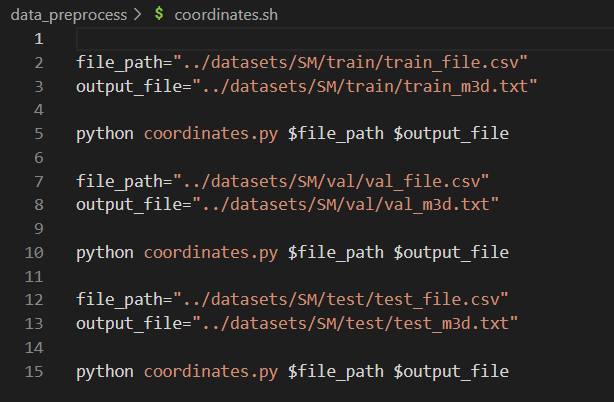
\includegraphics[width=0.6\textwidth]{GuideUtilisateur/coordinates1.png}
    \caption{Contenu du script coordinates.sh}
\end{figure}

Sur l'image on peut voir que chaque variable \texttt{file\_path} correspond au fichier créé lors de la séparation du dataset tandis que les variables \texttt{output\_path} correspondent aux fichiers de sortie qui contiendront les coordonnées 3D des molécules.

\subsection{Préparation des données pour le modèle} 

La troisième étape du projet consiste à préparer les données pour le modèle QDF. Pour cela, on utilise le script \texttt{preprocess.sh} qui se trouve dans le dossier \texttt{model/preprocess}.

\begin{figure}[H]
    \centering
    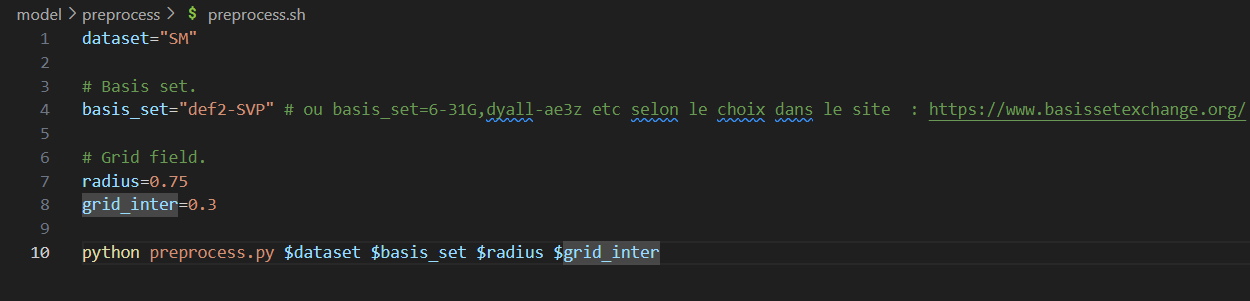
\includegraphics[width=0.8\textwidth]{GuideUtilisateur/preprocess1.png}
    \caption{Contenu du script preprocess.sh}
\end{figure}

La première variable \texttt{dataset} sert à définir le nom du dataset surlequel on souhaite faire du preprocessing. 
La deuxième variable \texttt{basis\_set} sert à définir l'ensemble de fonctions de bases utilisé.
Les variables \texttt{radius} et \texttt{grid\_size} servent à définir le rayon et la taille de la grille utilisée pour le champ électrique associé à chaque atomes.

\subsection{Entrainement du modèle}

La quatrième étape du projet consiste à entrainer le modèle QDF. Pour cela, on utilise le script \texttt{QDF\_SM.sh} ou \texttt{QDF\_PM.sh} qui se trouve dans le dossier \texttt{model/train\_model}.
Un ensemble de plusieurs paramètres sont à définir dans le script \texttt{QDF\_SM.sh} ou \texttt{QDF\_PM.sh} :

\begin{figure}[H]
    \centering
    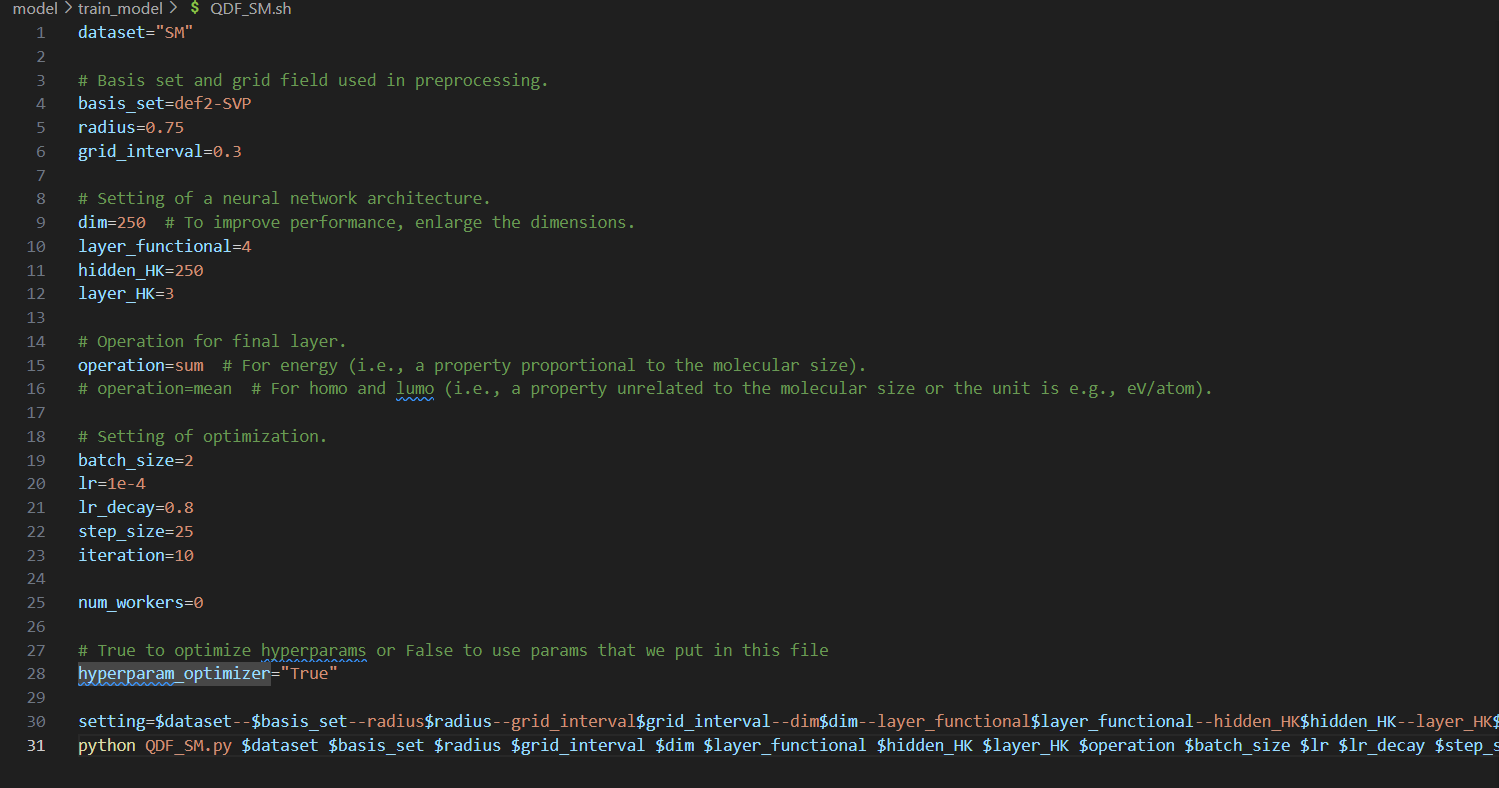
\includegraphics[width=0.8\textwidth]{GuideUtilisateur/train1.png}
    \caption{Variable contenu dans QDF\_SM.sh}
\end{figure}

Une variable importante qui influence la façon dont le modèle va apprendre est \texttt{hyperparam\_optimizer}.
Les hyperparamètres sont enregistrés dans un fichier qui servira de transfert learning pour l'entrainement du modèle QDF pour les PM.

\begin{figure}[H]
    \centering
    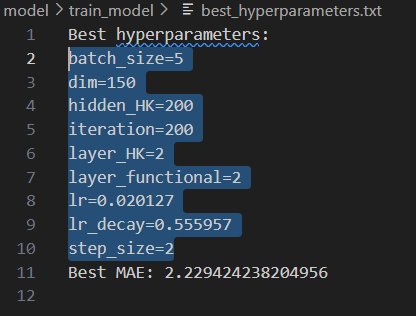
\includegraphics[width=0.3\textwidth]{GuideUtilisateur/hyper1.png}
    \caption{Hyperparamètres optimisés}
\end{figure}

On utilise les hyperparamètres optimisés pour le modèle QDF sur les SM pour entrainer le modèle QDF sur les PM.

\begin{figure}[H]
    \centering
    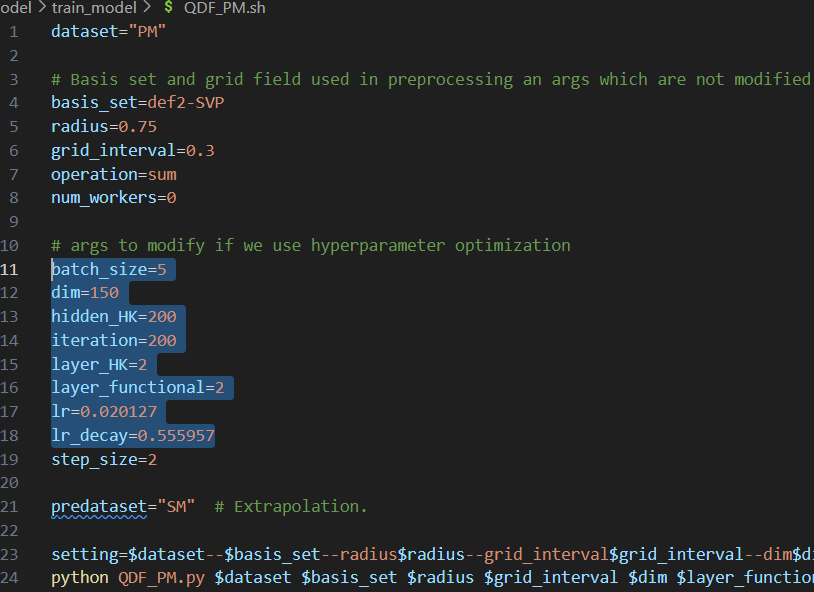
\includegraphics[width=0.6\textwidth]{GuideUtilisateur/pm1.png}
    \caption{Variable contenu dans QDF\_PM.sh}
\end{figure}

Il suffit juste de faire un copier de la partie surligner dans le fichier des hyperparamètres générés lors de l'entrainement du modèle QDF sur les SM et de le coller dans le fichier QDF\_PM.sh.
Les modèles d'entrainement sont sauvegardés dans le dossier \texttt{datasets/output}.

\subsection{Prédiction du PCE}

La dernière étape du projet pour le modèle de prédiction consiste à prédire le PCE des PM et SM grâce au modèle qu'on a pu entrainer. Pour cela, on utilise le script \texttt{predict.sh} qui se trouve dans le dossier \texttt{model/predict}.
Avant cela, il y a un prétraitement de données à faire , si les données reçues sont sous forme de SMILES, avec le script \texttt{preprocess\_predict.sh} se trouvant dans le même répertoire que \texttt{model/predict}. 

\subsection{Courbe d'apprentissage}

La courbe d'apprentissage est un outil essentiel pour évaluer la performance d'un modèle au fil du temps. 
Pour pouvoir la visualiser, il faut exécuter script python \texttt{courbe\_apprentissage.py} qui se trouve à la racine. 
Avant de le faire il faudrait s'assurer que le fichier \texttt{output\_SM.txt ou output\_PM.txt} contiennent des données si ce n'est pas le cas il faut aller dans dossier \texttt{datasets/output} et faire un copier-coller du fichier \texttt{SM--def2-SVP--radius0.75...} dans output\_SM.txt ou output\_PM.txt.

\begin{figure}[H]
  \centering
  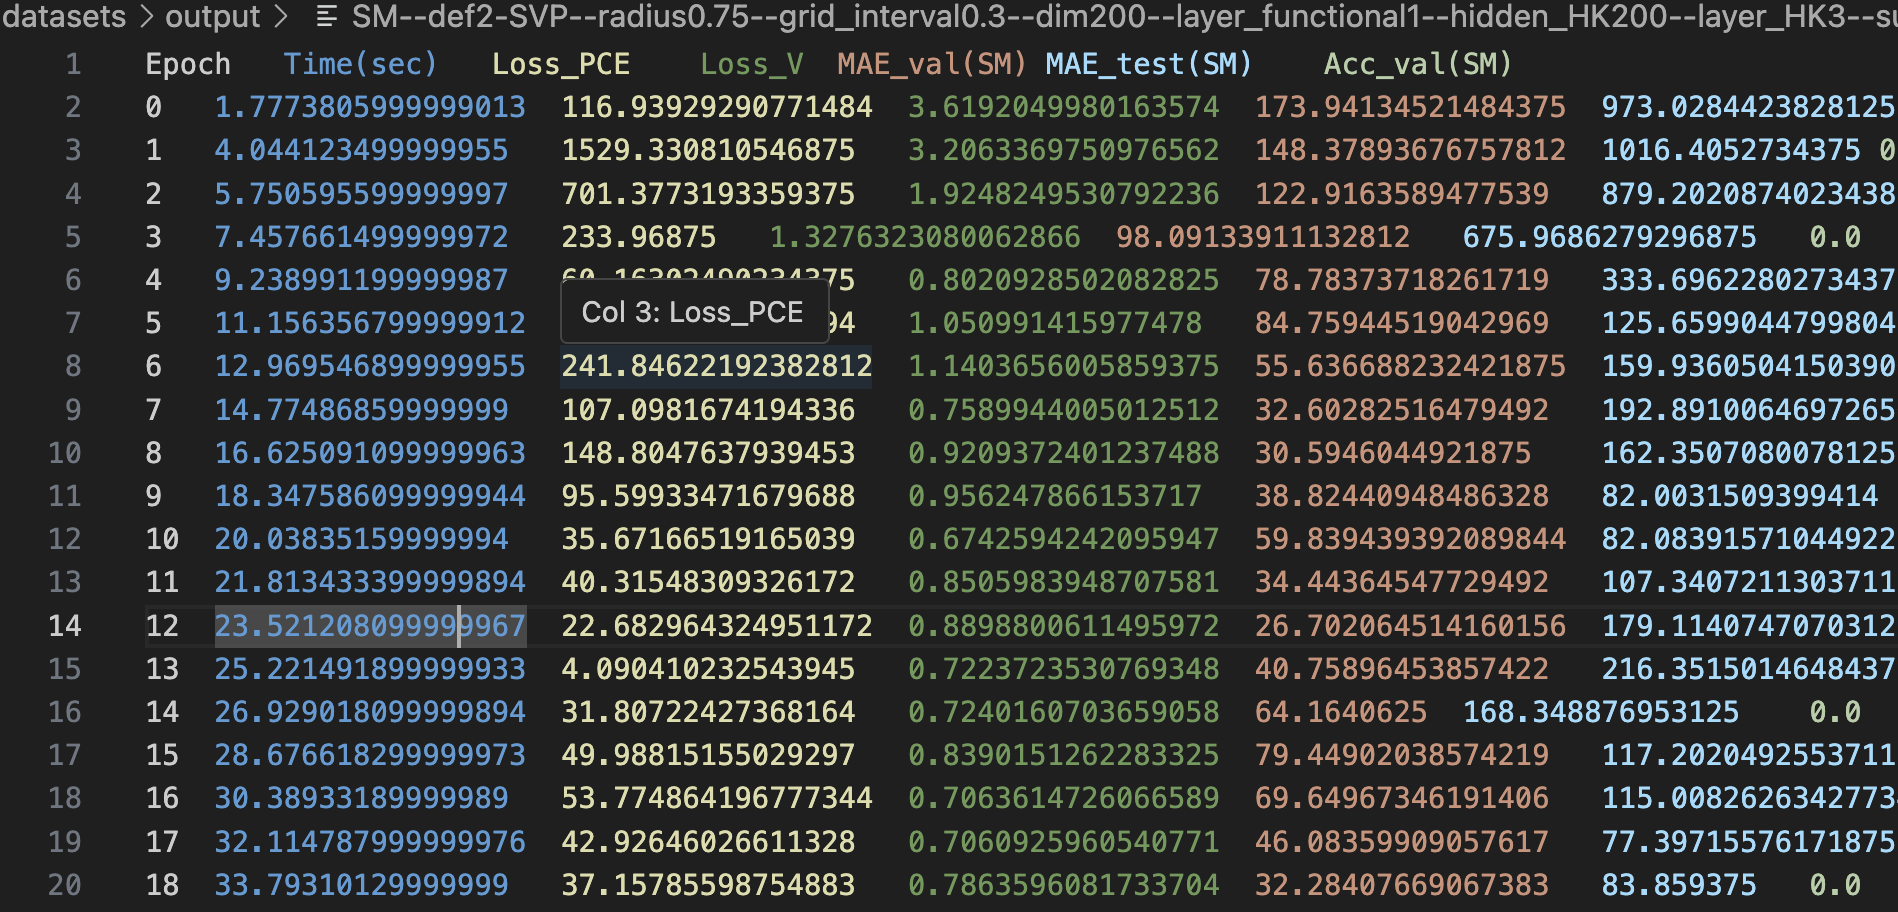
\includegraphics[width=0.6\textwidth]{GuideUtilisateur/train2.png}
  \caption{Contenu des données d'entrainement de datasets/ouput à copier-coller}
\end{figure}

On peut voir sur le graphe que les métrics utilisés pour ce modèle sont la perte et l'accuracy.

\subsection{Demo pour le modèle de prédiction}

En ce qui concerne la démo pour le modèle de prédiction, l'utilisateur pourra exécuter les fichiers \texttt{.ipynb} qui se trouvent dans les dossiers \texttt{data\_preprocess} et \texttt{model/preprocess} dans l'ordre des étapes décrites précédemment.
Une fois traitement des données réalisés une autre notebook présent dans le dossier \texttt{model/train\_model} sert uniquement à expliquer certaines composantes du projet. 
Pour avoir une démonstration de l'entrainement, faire du transfert learning et prédire il faudrait alors utiliser les scripts \texttt{QDF\_SM.sh} et \texttt{QDF\_PM.sh} qui se trouvent dans le dossier \texttt{model/train\_model} ainsi que ceux dans le dossier \texttt{predict}.

\subsection{VAE}
Le pipeline d'entraînement est structuré en plusieurs modules opérationnels :

\begin{itemize}
    \item \textbf{Chargement et nettoyage} : lecture des fichiers, suppression des erreurs et normalisation.
    \item \textbf{Encodage vectoriel} : transformation des SMILES en séquences compatibles avec le réseau neuronal.
    \item \textbf{Modélisation} : apprentissage d'une représentation latente des molécules à l'aide d'un modèle génératif.
    \item \textbf{Prédiction} : estimation de la Power Conversion Efficiency (PCE) en sortie du modèle.
    \item \textbf{Analyse et visualisation} : évaluation des performances, affichage graphique, génération de nouvelles structures.
\end{itemize}

Pour pourvoir exécuter le modèle, il faur se rendre dans le dossier \texttt{VAE} et exécuter le script \texttt{vae\_essaie.py} qui se trouve dans ce dernier depuis un terminal bash avec \texttt{python vae\_essaie.py} en activant l'environnement virtuel avant.
Un notebook est présent pour expliquer les fonctions du modèle en plus des commentaires.

% En lisant cette section, le lecteur devrait être en mesure de comprendre comment utiliser le modèle QDF pour prédire les propriétés des matériaux donneurs, en particulier le PCE. 
% Maintenant nous allons vous donnez une vue d'ensemble sur les libraries utilisé et le code pour ce projet.


\subsection{Conseils d'utilisation}

\subsubsection{GPU}
Lors de l'entrainement du modèle de prédiction, il est crucial d'utiliser un GPU suffisamment puissant et de disposer d'une quantité de mémoire RAM adaptée, que ce soit sur un PC personnel ou sur un serveur distant. En effet, l'entraînement de modèles de deep learning, en particulier sur des jeux de données volumineux ou des architectures complexes, nécessite des ressources matérielles importantes pour garantir des temps de calcul raisonnables et permettre l'utilisation de batchs de grande taille.
Pour l'entrainement de notre modèle de prédiction on a utilisé un server en ligne (OVHCloud) avec une \textbf{NVIDIA L40 S} avec 45 Go de mémoire GPU. 

\subsubsection{Basis set}
Le choix de la base de fonction est important pour la prédiction du PCE. 
Pour ce projet on a utilisé la base de fonction \textbf{def2-SVP} mais il est possible de le changer en fonction de la préférence. 
On l'a utilisé dans ce projet, car il couvrait un grand nombre d'élément chimique et est plus précis que le \textbf{6-31G}.

